\part[author={\protect\insertauthor},label={chap:lexical_analysis}]{Lexical Analysis}

\begin{graphicspathcontext}{{./chapters/chapter1/imgs/auto/},{./chapters/chapter2/imgs/auto/},{./chapters/chapter2/imgs/raw/}}
\begin{bibunit}[apalike]
	
\tableofcontentslide

\section{Introduction}
\sectiontableofcontentslide

\subsection{General principles}

\begin{rightlawnframe}<2>{Lexical Analyser}{lexical-analyzer-introduction}
	\putat*(340,-197){\includeanimatedfigure[width=2.5cm]{compiler_structure}}
	The lexical analyzer reads source program and extract lexemes \\[1cm]
	Each lexeme is associated to a token: \\
	\ccode{{\textless}token-name, \\
	\ attribute-value{\textgreater}} \\[1cm]
	Outputs the tokens
\end{rightlawnframe}

\begin{frame}{{Process of the} Lexical Analyzer}
	\begin{columns}
		\begin{column}{.5\linewidth}
			\begin{rightanchorblock}{}{1}
				Discovering the tokens
			\end{rightanchorblock}
			\begin{rightanchorblock}{}{2}
				Stripping the blanks and the comments
			\end{rightanchorblock}
			\begin{rightanchorblock}{}{3}
				Correlating the error messages with the source program (line number tracking\dots)
			\end{rightanchorblock}
		\end{column}
		\begin{column}{.5\linewidth}
			\begin{block}{Cascading Process (most of the time)}
				\begin{enumerate}
					\item[Scanning] processes that do not require tokenization of the input, e.g. deletion of comments and compaction of consecutive white spaces
					\item[Lexical analysing] produces tokens from the output of the scanner
				\end{enumerate}
			\end{block}
		\end{column}
	\end{columns}
\end{frame}

\subsection{Definitions}
\subsectiontableofcontentslide

\begin{frame}{Lexeme}
	\begin{definition}
		A sequence of characters in the source program that is identified by the lexical analyzer as a lexical unit (element of the language)
	\end{definition}
	\vspace{1cm}
	\begin{example}
		\begin{itemize}
		\item Let the statement: \code{printf("Total = \%d\n", score);}
		\item Both \code{printf} and \code{score} are lexemes
		\item String of characters is a lexeme
		\item Parenthesis, coma and semicolumn characters are also lexemes
		\end{itemize}
	\end{example}
\end{frame}

\begin{frame}{Token}
	\begin{definition}
		A pair consisting of a token \emph{name} and an optional \emph{attribute value}
		\begin{itemize}
			\item name: abstract symbol representing a kind of lexical unit
			\item token names are the input symbols that the parser processes
			\item token name is written in \token{bold-face}
		\end{itemize}
	\end{definition}
	\vfill
	\begin{example}
		\begin{itemize}
		\item Let the statement: \code{printf("Total = \%d\n", score);}
		\item both \code{printf} and \code{score} are lexemes matching the pattern for token \token{id}
		\end{itemize}
	\end{example}
\end{frame}

\begin{frame}{Pattern}
	\begin{definition}
		A description of the form that the lexemes of a token may take
		\begin{itemize}
			\item For keyword: the pattern is a sequence of characters that form the keyword
			\item For identifier and some other token: the pattern is a more complex structure that is \emph{matched} by many strings
		\end{itemize}
	\end{definition}
	\vspace{1cm}
	\begin{example}
		\begin{itemize}
		\item Let the statement: \code{printf("Total = \%d\n", score);}
		\item both \id{printf} and \id{score} are described by the pattern \regex{[\_a-zA-Z][\_a-zA-Z]*} (regex)
		\end{itemize}
	\end{example}
\end{frame}

\begin{frame}{Classes of Tokens}
	In many programming languages, the following classes cover most or all of the tokens: \\[.5cm]
	\begin{tabularx}{\linewidth}{|l|X|}
		\hline
		\tabularheading\chead{Class} & \chead{Description} \\
		\hline
		\token{keyword} & Pattern is the name of the token itself \\
		\hline
		\token{operator} & Individually or in classes, e.g., class \token{comparison} \\
		\hline
		\token{identifier} & One token per identifier \\
		\hline
		\token{constant} & One token per type of constant, e.g. number or string literal \\
		\hline
		\token{punctuation} & One token per punctuation symbol, e.g. left and right parentheses, comma, and semicolon \\
		\hline
	\end{tabularx}
\end{frame}

\begin{frame}{Attribute of Token}
	\begin{definition}
		Additional information associated to a token, when more than one lexeme can match a pattern
	\end{definition}
	\vspace{.5cm}
	\begin{examples}
		\begin{itemize}
		\item value of the parsed number (lexeme) for token \token{number}
		\item position of the identifier into the symbol table for token \token{id}
		\end{itemize}
	\end{examples}
	\vspace{.5cm}
	\begin{alertblock}{Assumption}
		Usually, token has at most one associated attribute; but it could be a data structure
	\end{alertblock}
\end{frame}

\subsection{Separating the lexical analyzer and the parser}
\subsectiontableofcontentslide

\begin{frame}{Relation between the Lexical Analyzer and the Parser}
	\alertbox*{Lexical analyzer generally does not control the execution flow of the compiler}
	\vspace{.5cm}
	\begin{center}
		\pgfuseimage{lexical-parser-relation}
	\end{center}
	\vspace{.5cm}
	\begin{itemize}
	\item Lexical analyzer is invoked by the parser through a call to \code{getNextToken} function
	\item Then, lexical analyzer tries to discover and to reply a token
	\end{itemize}
\end{frame}

\begin{frame}{{Why Separating} Lexical Analyzer and Parser?}
	\fancybox{Design Simplicity}{Enable simplification of at least one of these tasks}{software-design}{1}
	\hfill
	\fancybox{Compiler Efficiency}{Enable application of specialized techniques}{software-efficiency}{2}
	\hfill
	\fancybox{Easier Portability}{Specific input devices supported by lexical analyzer}{software-portability}{3}
\end{frame}

\subsection{Lexical errors}
\subsectiontableofcontentslide

\begin{frame}[t]{Lexical Errors}
	\alertbox{It is hard for a lexical analyzer to tell that there is a source-code error}
	\vspace{.25cm}
	\begin{example}
		\code{fi ( a == f(x) ) ...}
	\end{example}
	\vspace{.25cm}
	\begin{alertblock}{Problems}
		\begin{itemize}
		\item Cannot tell whether \code{fi} is a misspelling of the keyword \code{if} or an undeclared function identifier
		\item Fails when none of the patterns for tokens matches any prefix of the remaining input
		\end{itemize}
	\end{alertblock}
	\vspace{.25cm}
	\alertbox*{If such an error is detected, lexical analyzer must output an error message \\
		and try to \emph{recover} a stable state}
\end{frame}

\begin{leftlawnframe}{{Recovery Strategy:} Panic Mode}{panic-mode}
	Successive characters are deleted from the remaining input, until the lexical analyzer can find a well-formed token at the beginning of input
\end{leftlawnframe}

\begin{gridframe}{{Other} Recovery Strategies}
	\cell2{delete-icon}{\small Delete character from input}
	\cell4{insert-icon}{\small Insert character into input}
	\cell7{replace-icon}{\small Replace character in input}
	\cell9{transpose-icon}{\small Transpose adjacent characters}
\end{gridframe}

\section{Input buffering}
\sectiontableofcontentslide

\begin{frame}{Reading the Source Program}
	\begin{rightarrowsequence}
		\arrow[decoration=icon-goal]{Reading input is key task that must be efficient}
		\arrow[bg=CIADmagenta, decoration=icon-problem]{Have to look one or more characters beyond the next lexeme to extract the right lexeme}
		\arrow[bg=CIADgreen, decoration=icon-solution]{Two-buffer scheme that handles large lookaheads safely}
	\end{rightarrowsequence}
	\vspace{.25cm}
	\begin{example}
		To be sure that a character is the last of an identifier, the next character must be read, and it is not part of the lexeme for \token{id}
	\end{example}
\end{frame}

\begin{frame}{Principles of the Two-Buffer Scheme}
	\alertbox*{Two buffers are read and used alternatively}
	\begin{center}
		{\pgfuseimage{buffer_pair_example}}
	\end{center}
	\vspace{.25cm}
	\begin{description}
		\item[Assumption] the larger lexeme has a size lower or equals to $N$
		\item $N$ is usually the size of the disk block
		\item \token{eof} character is put in the buffer when there is not enough characters in the input
	\end{description}
	\vspace{1cm}
	\simplebox{\Emph{How to be efficient?} By invoking the \code{read} system function for $N$ characters rather than a call per character}
\end{frame}

\begin{frame}[t]{{Two Reading} Pointers}
	\begin{center}
		{\pgfuseimage{buffer_pair_example1}}
	\end{center}
	\begin{itemize}
	\item \id{lexemeBegin}: the beginning of the current lexeme
	\item \id{forward}: the current character
	\end{itemize}
	\vspace{.25cm}
	\begin{block}{Algorithmic Principle}
		\begin{enumerate}
			\item \emph{If \id{forward} is outside a buffer}, the other buffer is reloaded from the input, and move \id{forward} to the beginning of the newly loaded buffer
			\item \emph{If character pointed by \id{forward} does not match a lexeme from \id{lexemeBegin}}:
				\begin{itemize}
					\item \emph{If it is a valid lexeme}, output the lexeme, move \id{lexemeBegin} to \id{foward}
					\item \emph{Else} generate an error
				\end{itemize}
			\item \emph{Else} move \id{forward} to the right
		\end{enumerate}
	\end{block}
\end{frame}

\begin{frame}{{Be More Efficient} with Sentinels}
	\begin{alertblock}{Problem of efficiency}
		For each character read, two tests: \begin{enumerate}
		\item one for the end of the buffer
		\item one to determine what character is read (usually with a multiway branch)
		\end{enumerate}
	\end{alertblock}
	\vspace{.5cm}
	$\Rightarrow$ To improve the speed of the treatment, we can combine the two tests by extending each buffer with a \emph{sentinel character} (usually \token{eof}) \\
	\vspace{.5cm}
	\begin{center}
		\pgfuseimage{buffer_pair_sentinel_example}
	\end{center}
\end{frame}

\begin{frame}{{Can We Run Out Of} Buffer Space?}
	\begin{rightarrowsequence}
		\arrow{
			In most modern languages, lexemes are short \\
			$N \ge 1000$ is ample
		}
		\arrow[bg=CIADmagenta, decoration=icon-problem]{
			Character strings can be very long (more than $N$)
		}
		\arrow[bg=CIADgreen, decoration=icon-solution]{
			Add a dynamic buffer scheme for large lexeme
		}
		\arrow[bg=CIADgreen, decoration=icon-solution]{
			Reply a sequence of \token{str} tokens, one for each of the shorter strings (see example)
		}
	\end{rightarrowsequence}
	\begin{example}
		Compile-time string concatenation in C: \code{"ABC" "DEF"}
	\end{example}
\end{frame}


\section[Token Recognition]{Specification and recognition of tokens}
\sectiontableofcontentslide

\subsection{Definitions and operations on languages}
\subsectiontableofcontentslide

\begin{frame}{Definitions of Alphabet, String and Language}
	\begin{definitionblock}{Alphabet}
		Any finite set of symbols; \inlineexample{$A = \left\{a,b,c,\delta\right\}$}
	\end{definitionblock}
	\vspace{.25cm}
	\begin{definitionblock}{String}
		A finite sequence $s$ of symbols drawn from an alphabet $A$. \\
		\inlineexample{$s \in S / S = \permut(\powerset(A)) \setminus \{\emptyset\} = \left\{a,b,c,\delta,ab,ac,a\delta,\dots\right\}$} \\
		$|s|$ is the size of $s$
	\end{definitionblock}
	\vspace{.25cm}
	\begin{definitionblock}{Language}
		Any countable set of strings over some fixed alphabet \\
		\inlineexample{$L \subseteq S = \left\{abc,\delta,b,bc\right\}$}
		%	\end{itemize}
	\end{definitionblock}
\end{frame}

\sidecite{Kleene.1956}
\begin{frame}{Operations on Languages}
	\alertbox*{The following operations are used for defining the pattern matchings for languages}
	\vspace{1cm}
	\begin{block}{Union of the languages $L$ and $M$}
		$L \cup M = \left\{s | s\in L \vee s \in M\right\}$
		\begin{tabularx}{\linewidth}{@{}lX@{}}
		\insertexamplelabel & Let $L = \left\{ a, b ,c \right\}$ and $M = \left\{ d, e \right\}$ \\
		& then $L \cup M = \left\{ a, b, c, d, e \right\}$
		\end{tabularx}
	\end{block}
	\vspace{.5cm}
	\begin{block}{Concatenation of the languages $L$ and $M$}
		$LM = \left\{st | s\in L, t \in M\right\}$
		\begin{tabularx}{\linewidth}{@{}lX@{}}
		\insertexamplelabel & Let $L = \left\{ a, b ,c \right\}$ and $M = \left\{ d, e \right\}$ \\
		& then $LM = \left\{ ad, ae, bd, be, cd, ce \right\}$
		\end{tabularx}
	\end{block}
\end{frame}

\sidecite{Kleene.1956}
\begin{frame}{Operations on Languages \insertcontinuationtext}
	\begin{block}{Self-concatenation of the language $L$}
		$L^i = \begin{cases}
			\{\epsilon\} & \text{if }i=0 \\
			L^{i-1}L & \text{if }i>0 \\
			\end{cases}$
		\begin{tabularx}{\linewidth}{@{}lX@{}}
		\insertexamplelabel & Let $M = \left\{ d, e \right\}$ \\
		& then $M^4 = \left\{ \begin{array}{llllll}
			\scriptstyle dddd, & \scriptstyle ddde, & \scriptstyle dded, & \scriptstyle ddee, \\
			\scriptstyle dedd, & \scriptstyle dede, & \scriptstyle deed, & \scriptstyle deee, \\
			\scriptstyle eddd, & \scriptstyle edde, & \scriptstyle eded, & \scriptstyle edee, \\
			\scriptstyle eedd, & \scriptstyle eede, & \scriptstyle eeed, & \scriptstyle eeee \end{array} \right\}$
		\end{tabularx}
	\end{block}
\end{frame}

\sidecite{Kleene.1956}
\begin{frame}[c]{Operations on Languages \insertcontinuationtext}
	\begin{block}{Kleene's Closure of the language $L$}
		$L^* = \bigcup^{\infty}_{i=0}L^i$
		\begin{tabularx}{\linewidth}{@{}lX@{}}
		\insertexamplelabel & Let $M = \left\{ d, e \right\}$ \\
		& then $M^* = \left\{ \begin{array}{l}
			\scriptstyle \epsilon, d, e, dd, de, ed, ee, ddd, dde, ded, dee, edd, ede, eed, \\
			\scriptstyle eee, dddd, ddde, dded, ddee, dedd, dede, deed, deee, \dots\end{array} \right\}$
		\end{tabularx}
	\end{block}
	\vspace{.5cm}
	\begin{block}{Positive Closure of the language $L$}
		$L^+ = \bigcup^{\infty}_{i=1}L^i$
		\begin{tabularx}{\linewidth}{@{}lX@{}}
		\insertexamplelabel & Let $M = \left\{ d, e \right\}$ \\
		& then $M^+ = \left\{ \begin{array}{l}
			\scriptstyle d, e, dd, de, ed, ee, ddd, dde, ded, dee, edd, ede, eed, \\
			\scriptstyle eee, dddd, ddde, dded, ddee, dedd, dede, deed, \dots\end{array} \right\}$
		\end{tabularx}
	\end{block}
\end{frame}

\subsection{Regular expressions}
\subsectiontableofcontentslide

\sidecite{Kleene.1956, Shannon.1956, Aho.1990, Aho.1988}
\begin{frame}{Regular Expressions}
	\begin{definitionblock}{Regular Expressions (shortened as regex, regexp or rational expression)}
		A sequence of characters that specifies a search pattern.
	\end{definitionblock}
	\vspace{.5cm}
	\begin{rightarrowsequence}
		\arrow{Usually used for describing all the languages that can be built from the operators previously defined}
		\arrow{
			Built recursively out of smaller regular expressions (see following slides). \\[.25cm]
			Each regular expression $r$ denotes a language $L(r)$, which is also defined recursively from the languages denoted by $r$'s expressions.
		}
	\end{rightarrowsequence}
\end{frame}

\begin{frame}{Basis of Regular Expressions}
	The rules that define the regular expressions over some alphabet $\Sigma$ and the languages that those expressions denote are:
	\vspace{.25cm}
	\begin{definition}[BASIS]
	There are two rules that form the basis: \begin{enumerate}
	\item $\epsilon$ is a regular expression, and $L(\epsilon)$ is $\{\epsilon\}$, that is, the language whose sole member is the empty string.
	\item If a is a symbol in $\Sigma$, then \regex{a} is a regular expression, and $L(\regex{a}) = \{a\}$, that is, the language with one string, of length one, with $a$ in its position.
	\end{enumerate}
	\end{definition}
	\vspace{.25cm}
	\begin{block}{\smaller Remark}\smaller 
		By convention, we use \textit{italics} for symbols, and \regex{boldface} for their corresponding regular expressions.
	\end{block}
\end{frame}

\begin{frame}{Induction with Regular Expressions}
	\begin{definition}[INDUCTION]
	There are four parts to the induction whereby larger regular expressions are built from smaller ones. Suppose $r$ and $s$ are regular expressions denoting languages $L(r)$ and $L(s)$, respectively.
	\begin{enumerate}
	\item $(r)|(s)$ is a regular expression denoting the language $L(r) \cup L(s)$
	\item $(r)(s)$ is a regular expression denoting the language $L(r)L(s)$
	\item $(r)*$ is a regular expression denoting the language $(L(r))^*$
	\item $(r)$ is a regular expression denoting $L(r)$
	\end{enumerate}
	\end{definition}
	This last rule says that we can add additional pairs of parentheses around expressions without changing the language they denote.
\end{frame}

\begin{frame}{Simplification Conventions for Induction}
	\alertbox*{Regular expressions often contain unnecessary pairs of parentheses}
	\vspace{1cm}
	\begin{block}{Simplification Rules}
		\begin{enumerate}[a)]
			\item The unary operator "$*$" has highest precedence and is left associative.
			\item Concatenation has second highest precedence and is left associative.
			\item "$|$" has lowest precedence and is left associative.
		\end{enumerate}
	\end{block}
\end{frame}

\begin{frame}{Regular Set}
	\begin{definitionblock}{Regular Set}
		A language that can be defined by a regular expression \\
		\smaller If two regular expressions $r$ and $s$ denote the same regular set, they are equivalent $r = s$
	\end{definitionblock}
	\vspace{.5cm}
	\begin{tabularx}{\linewidth}{|X|X|X|}
		\hline
		\tabularheading\chead{Law}&\chead{Description} \\
		\hline
		$r|s = s|r$ & $|$ is commutative \\
		\hline
		$r|(s|t) = (r|s)|t$ & $|$ is associative \\
		\hline
		$r(st) = (rs)t$ & Concatenation is associative \\
		\hline
		$r(s|t) = rs|rt$; $(s|t)r = st|tr$ & Concatenation distributes over $|$ \\
		\hline
		$\epsilon r = r\epsilon = r$ & $\epsilon$ is the identity for concatenation \\
		\hline
		$r* = (r|\epsilon)*$ & $\epsilon$ is guaranteed in a closure \\
		\hline
		$r** = r*$ & $*$ is idempotent \\
		\hline
	\end{tabularx}
\end{frame}

\subsection{Regular definitions}
\subsectiontableofcontentslide

\begin{frame}[t]{Regular Definitions}
	\alertbox{For notational convenience, we may wish to give names to certain regular expressions and use those names in subsequent expressions, as if the names were themselves symbols}
	\vspace{.25cm}
	\begin{definitionblock}{Regular definition}
		If $\Sigma$ is an alphabet of basic symbols, a regular definition is a sequence of definitions of the form: \\
		\centering\begin{tabular}{rcl}
			\regex{d\textdown{1}} & $\rightarrow$ & $r_1$ \\
			\regex{d\textdown{2}} & $\rightarrow$ & $r2$ \\
			& \dots &\\
			\regex{d\textdown{n}} & $\rightarrow$ & $r_n$ \\
		\end{tabular}
		\begin{itemize}
			\item \regex{d\textdown{i}} is a new symbol, not in and not the same as any other of the $d$'s
			\item $r_i$ is a regular expression over the alphabet $\Sigma\cup\{\regex{d\textdown{1}},\regex{d\textdown{2}},\dots,\regex{d\textdown{i-1}}\}$.
		\end{itemize}
	\end{definitionblock}
\end{frame}

\begin{frame}[background=8]{Well-known Regular Definitions}
	\centering
	\begin{tabular}{rcl}
		\regex{letter} & $\rightarrow$ & $A | B | \dots | Z | a | b | \dots | z$ \\[.2cm]
		\regex{letter\_} & $\rightarrow$ & $\regex{letter} | \_$ \\[.2cm]
		\regex{digit} & $\rightarrow$ & $0 | 1 | \dots | 9$ \\[.2cm]
		\regex{letters} & $\rightarrow$ & $\regex{letter}\ \regex{letter}*$ \\[.2cm]
		\regex{digits} & $\rightarrow$ & $\regex{digit}\ \regex{digit}*$ \\[.2cm]
		\regex{id} & $\rightarrow$ & $\regex{letter\_} ( \regex{letter\_} | \regex{digit} )*$ \\[.2cm]
		\regex{optFrac} & $\rightarrow$ & $.\ \regex{digits} | \epsilon$ \\[.2cm]
		\regex{optExp} & $\rightarrow$ & $( (E|e) (+|-|\epsilon) \regex{digits} ) | \epsilon$ \\[.2cm]
		\regex{number} & $\rightarrow$ & \regex{digits}\ \regex{optFrac}\ \regex{optExp} \\
	\end{tabular}
\end{frame}

\sidecite{Kleene.1956}
\begin{frame}[t]{Extension of the Regular Definitions}
	\alertbox*{Since \cite{Kleene.1956} introduced regular expressions with the basic operators in 1950s, many extensions have been added to enhance their ability to specify string patterns}
	\vspace{.25cm}
	\fancybox{One or more instances}{
		$L(r+) = (L(r))^+$ \\
		Same precedence and associativity as "$*$"}{rplus_regex}{1}
	\hfill
	\fancybox{Zero or one instance}{
		$L(r?) = L(r)\cup\{\epsilon\}$ \\
		Same precedence and associativity as "$*$"}{rquestionmark_regex}{2}
	\hfill
	\fancybox{Character classes}{
		$[ab{\ldots}z] = a|b|\ldots|z$ \\
		Consecutive symbols: $[a-z]$}{class_regex}{3}
\end{frame}

\begin{frame}[background=8]{Revision of the Regular Definitions}
	\centering
	\begin{tabular}{rcl}
		\regex{letter} & $\rightarrow$ & $[A-Za-z]$ \\[.2cm]
		\regex{letter\_} & $\rightarrow$ & $[A-Za-z\_]$ \\[.2cm]
		\regex{digit} & $\rightarrow$ & $[0-9]$ \\[.2cm]
		\regex{letters} & $\rightarrow$ & $\regex{letter}+$ \\[.2cm]
		\regex{digits} & $\rightarrow$ & $\regex{digit}+$ \\[.2cm]
		\regex{id} & $\rightarrow$ & $\regex{letter\_} ( \regex{letter\_} | \regex{digit} )*$ \\[.2cm]
		\regex{number} & $\rightarrow$ & $\regex{digits} (. \regex{digits})? ([Ee][+-]? \regex{digits})?$ \\
	\end{tabular}
	\[\begin{array}{@{}ll@{}}
		
	\end{array}\]
\end{frame}

\subsection{Recognition of tokens}

\subsubsection{Definition of the Lexeme-Token Pairs}
\subsubsectiontableofcontentslide*

\begin{frame}{Definition of our Illustrative Language}
	\alertbox*{We are able to express patterns using regular expressions \\
		How to define regex patterns for all the tokens of our language?}
	\vspace{.5cm}
	\centering
	\begin{tabular}{rcl}
		\regex{statement} & $\rightarrow$ & \ccode{\kw{if}} \regex{expr} \ccode{\kw{then}} \regex{statement} \ccode{\kw{else}} \regex{statement} \\
		& $\rightarrow$ & \regex{term} \\[.2cm]
		\regex{expr} & $\rightarrow$ & \regex{term} \ccode{=} \regex{term} \\
		& $\rightarrow$ & \regex{term} \ccode{{\textless}{\textgreater}} \regex{term} \\
		& $\rightarrow$ & \regex{term} \ccode{\textless} \regex{term} \\
		& $\rightarrow$ & \regex{term} \ccode{\textgreater} \regex{term} \\
		& $\rightarrow$ & \regex{term} \ccode{\textless=} \regex{term} \\
		& $\rightarrow$ & \regex{term} \ccode{\textgreater=} \regex{term} \\[.2cm]
		\regex{term} & $\rightarrow$ & \regex{number} \\
		& $\rightarrow$ & \regex{id} \\
	\end{tabular}
\end{frame}

\begin{frame}{Definition of the Lexeme-Token Pairs}
	\begin{small}
	\begin{tabularx}{\linewidth}{|l|X|l|X|}
		\hline
		\tabularheading\chead{Lexeme}&\chead{Regular Expression}&\chead{Token}&\chead{Token Attributes} \\
		\hline
		ws & $[\ {\backslash}n{\backslash}t{\backslash}r]+$ & - & - \\
		\hline
		if & $if$ & \token{if} & - \\
		\hline
		then & $then$ & \token{then} & - \\
		\hline
		else & $else$ & \token{else} & - \\
		\hline
		id & $\regex{letter\_}\ (\regex{letter\_}|\regex{digit})*$ & \token{id} & pointer to symbol table's entry \\
		\hline
		number & $\regex{digits}(.\ \regex{digits})?$ & \token{number} & pointer to symbol table's entry \\
		\hline
		= & $=$ & \token{relop} & \ccode{EQ} \\
		\hline
		{\textless}{\textgreater} & $<>$ & \token{relop} & \ccode{NE} \\
		\hline
		{\textless} & $<$ & \token{relop} & \ccode{LT} \\
		\hline
		{\textgreater} & $>$ & \token{relop} & \ccode{GT} \\
		\hline
		{\textless}= & $<=$ & \token{relop} & \ccode{LE} \\
		\hline
		{\textgreater}= & $>=$ & \token{relop} & \code{GE} \\
		\hline
	\end{tabularx}
	\end{small}
\end{frame}

\subsubsection{Transition Diagram}
\subsubsectiontableofcontentslide

\begin{frame}[t]{Transition Diagram}
	As an intermediate step in the construction of a lexical analyzer, patterns are converted to flowcharts, called \emph{transition diagrams}.
	\vspace{.5cm}
	\begin{definition}[Transition Diagram]
	\begin{description} 
	\item[Diagram] composed of states and edges
	\item[State] a step in the scanning of a string, that also indicates if the input stream is validating the regular expression, or not
	\item[Edge] directed from one state to another. Each edge is labeled by a symbol or a set of symbols
	\end{description}
	\end{definition}
	\begin{alertblock}{Assumption}
	All transition diagrams are deterministic: never more than one edge out of a given state with a given symbol among its labels.
	\end{alertblock}
\end{frame}

\begin{frame}{Specific Notations}
	\begin{small}
		\begin{tabularx}{\linewidth}{|c|X|}
			\hline
			\tabularheading\chead{Notation}&\chead{Explanation} \\
			\hline
			\raisebox{-.7\height}{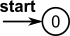
\includegraphics[width=4em]{transition_diagram_start}} &  The transition diagram always begins in the \emph{start state} before any input symbols have been read. \\
			\hline
			\raisebox{-.8\height}{
\includegraphics[width=5em]{transition_diagram_other}} &  The transition labelled with \textbf{other} is traversable when no other transition is traversable. \\
			\hline
			\raisebox{-.7\height}{
\includegraphics[width=1.7em]{transition_diagram_accept_state}} & The \emph{accepting state} (or final) indicates that a lexeme has been found (between pointers \code{lexemeBegin} and \code{forward}).
			\\
			\hline
			\raisebox{-\height}{
\includegraphics[width=2em]{transition_diagram_retract_state}} & If the lexeme does not include the symbol that got us to the accepting state, it is necessary to \emph{retract} the \code{forward} pointer by one position. \\
			\hline
		\end{tabularx}
	\end{small}
\end{frame}

\figureslide{Example of a Transition Diagram for \token{relop}}{transition_diagram_relop}

\begin{frame}{Problem with Identifiers and Keywords}
	\begin{itemize}
	\item The transition diagram that recognizes the identifiers is:
	\vfill
		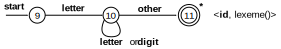
\includegraphics[width=\linewidth]{transition_diagram_identifier}
	\vfill
	\item \code{lexeme()} replies the current lexeme (between \code{lexemeBegin} and \code{forward} pointers).
	\end{itemize}
	\vfill
	\alertbox{Recognizing keywords and identifiers presents a specific problem:
keywords are not identifiers even though they look like identifiers.}
\end{frame}

\begin{frame}{{Solving the Problem} with Identifiers and Keywords}
	\simplebox{
		\raggedright\begin{tabularx}{\linewidth}{@{}lX}
		\textcircled{1} &
		Install all the keywords in the symbol table initially \newline
		A field of the symbol-table entry indicates that the string are never ordinary identifier
			\begin{itemize}
			\item \code{installID()} places the identifier in the symbol table if it is not already there and returns a pointer to the symbol-table entry.
			\item \code{getToken()} replies the token that is corresponding to the lexeme, or \token{id} otherwise.
			\end{itemize}
		\end{tabularx}
	}
	\vspace{.5cm}
	\pgfuseimage{transition_diagram_identifier_keyword}
\end{frame}

\begin{frame}{{Solving the Problem} with Identifiers and Keywords \insertcontinuationtext}
	\simplebox{
		\raggedright\begin{tabularx}{\linewidth}{@{}lX}
			\textcircled{2}&
			Create a separate transition diagram for each keyword
			\begin{itemize}
				\item tokens must be prioritized so that the reserved-word tokens are recognized in preference to \token{id}
				\item Approach less used than the previous approach when the lexical analyzer is written by hand
			\end{itemize}
		\end{tabularx}
	}
\end{frame}

\subsubsection{Implementation of a Lexical Analyzer based on Transition Diagrams}
\subsubsectiontableofcontentslide

\begin{frame}{Implementation of a Lexical Analyzer}
	\alertbox*{There are several ways that a collection of transition diagrams can be used to build a lexical analyzer}
	\begin{itemize}
	\item A variable state is holding the number of the current state for a transition diagram
	\vspace{.5cm}
	\item Each transition diagram is simulated by a piece of code inside a function
	\vspace{.5cm}
	\item The code of a state is itself a switch statement or a multiway branch that determines the next state by reading and examining the next input character.
	\end{itemize}
\end{frame}

\begin{frame}[t,fragile]{Example of Code for the Token \token{relop}}
	\begin{lstlisting}[style=lststyle-java]
Token getRelop() { /* return null on failure */
  char c;
  int state = 0;
  Token token = new Token(Tag.RELOP);
  while (true) { /* repeat until a return or failure */
    switch(state) {
    case 0: 
      c = nextChar();
      if (c=='<') state = 1;
      else if (c=='=') state = 5;
      else if (c=='>') state = 6;
      else return null; /* lexeme is not a relop */
      break;
    case 1: ...
    case 8:
      retract(); // move back the "forward" and "lexemeBegin" pointers
      token.attribute = "GT";
      return token;
    default: return null;
    }
  }
}
	\end{lstlisting}
\end{frame}

\begin{frame}{Combine Transition Diagrams}
	\alertbox*{To build the entire lexical analyzer, the codes for simulating the transition diagrams may be arranged in different ways}
	\vspace{.5cm}
	\simplebox{
		\raggedright\begin{tabularx}{\linewidth}{@{}lX}
			\textcircled{1} &
			Arrange for the transition diagrams for each token to be tried sequentially
			\begin{itemize}
				\item When the function is replying \code{null} (failure), the pointer \code{forward} is reset and the next transition diagram is started
				\item This approach allows us to use the \emph{transition diagrams for the individual keywords}
				\item We have only to use them \emph{before} we use the diagram for \token{id}, in order the keywords to be reserved words
			\end{itemize}
		\end{tabularx}
	}
\end{frame}

\begin{frame}{Combine Transition Diagrams \insertcontinuationtext}
	\simplebox{
		\raggedright\begin{tabularx}{\linewidth}{@{}lX}
			\textcircled{2} &
			Run the various transition diagrams ``in parallel''
			\begin{itemize}
				\item \emph{Caution:} be careful to resolve the case where one diagram finds a lexeme that matches its pattern, while one or more other diagrams are still able to process input
				\item \emph{Strategy:} take the longest prefix of the input that matches any pattern
			\end{itemize}
		\end{tabularx}
	}
\end{frame}

\begin{frame}{Combine Transition Diagrams \insertcontinuationtext}
	\simplebox{
		\raggedright\begin{tabularx}{\linewidth}{@{}lX}
			\textcircled{3} &
			Preferred approach: combine all the transition diagrams in one
			\begin{itemize}
				\item Transition diagram reads input until there is no possible next state
				\item Then, longest lexeme that matched any pattern is replied
			\end{itemize}
		\end{tabularx}
	}
	\vspace{.5cm}
	\alertbox{
		The problem of combining transition diagrams for several tokens is complex. \\
		The easiest way to solve this problem is to study how lexical-analyzer generators, such as Lex or Flex, are working
	}
\end{frame}

\section[Generators of lexical analyser]{Writing a lexical analyzer with Lex, Flex, JFlex, JavaCC}
\sectiontableofcontentslide

\sidecite{Lesk.1975}
\begin{frame}{Generators of Lexical Analyser}
	\alertbox*{Several tools allow to generate a lexical analyzer by specifying regular expressions to describe the patterns for the tokens}
	\begin{itemize}
	\item This section introduces the tool:
		\begin{itemize}
			\item Lex, and its more recent implementation Flex (dedicated to compilers written in C or C++)
			\item JavaCC (dedicated to compilers written in Java)
		\end{itemize} 
	\item The input notation is the Lex language
	\end{itemize}
	\vfill
	\pgfuseimage{lex_tool}
\end{frame}

\subsection{Lex Generator}

\subsubsection{Use of Lex}
\subsubsectiontableofcontentslide*

\figureslide{Process of Lex}{lex_process}

\begin{frame}[background=8]{{Key points} to Implement \ccode{main.c}}
	\begin{itemize}
		\item \emph{The lexical analyzer is a C function} that returns an integer, which is a code for one of the possible token names
		\vfill
		\item This \emph{subroutine} is called by the parser
		\vfill
		\item Attribute value (another numeric code) is a pointer to the symbol table, or nothing
		\item This value is placed in a global variable \code{yylval}
	\end{itemize}
\end{frame}

\subsubsection{Lex program}

\begin{frame}[t,fragile]{Structure of a Lex program}
	A Lex program has the following form:
		\begin{lstlisting}[language=python]
Declarations
%%
Translation rules
%%
Auxiliary functions
		\end{lstlisting}
	\only<1>{\begin{block}{Declarations}
		\begin{itemize}
		\item Declarations of variables (in C)
		\item Manifest constants: identifiers declared to stand for a constant, eg. the name of a token
		\item Regular definitions
		\end{itemize}
	\end{block}}
	\only<2>{\begin{block}{Translation rules}
		\begin{itemize}
		\item Have the form:
			\begin{center}
				\ccode{Pattern \{ Actions \}}
			\end{center}
		\item Pattern is a regex
		\item Actions are fragments of C code
		\item Evaluation order: first matching rule, first used
		\end{itemize}
	\end{block}}
	\only<3>{\begin{block}{Auxiliary functions}
		\begin{itemize}
		\item Holds whatever additional functions are used in the actions
		\end{itemize}
	\end{block}}
\end{frame}

\begin{frame}[fragile,background=9]{{Example of a Lex Program:} declarations}
	\begin{lstlisting}[style=lststyle-c]
%{
  /* definitions of manifest constants, if not already
     declared in the parser files (yacc) */
  enum { LT, LE, EQ, NE, GT, GE	} RelopId;
  enum { IF, THEN, ELSE, ID, NUMBER, RELOP } TokenName;
%}


/* regular expressions */
delim   [ \t\n]
ws      {delim}+
letter  [A-Za-z]
digit   [0-9]
id      {letter}({letter}|{digit})*
number  {digit}+(\.{digit}+)?([Ee][+-]?{digit}+)?

%%
	\end{lstlisting}
\end{frame}

\begin{frame}[fragile,background=6]{{Example of a Lex Program:} translation rules}
	\begin{lstlisting}[style=lststyle-c]
{ws}      { /* no action and no return */ }
if        { return IF; }
then      { return THEN; }
else      { return ELSE; }
{id}      { yylval = (int)installID(); return ID; }
{number}  { yylval = (int)installNumber(); return NUMBER; }
"<"       { yylval = LT; return RELOP; }
"<="      { yylval = LE; return RELOP; }
"="       { yylval = EQ; return RELOP; }
"<>"      { yylval = NE; return RELOP; }
">"       { yylval = GT; return RELOP; }
">="      { yylval = GE; return RELOP; }

%%
	\end{lstlisting}
\end{frame}

\begin{frame}[fragile,background={10}]{{Example of a Lex Program:} auxiliary functions}
	\begin{lstlisting}[style=lststyle-c]
int installID() {
  /* function to install the lexeme, whose first
     character is pointed to by yytext, and whose
     length is yyleng, into the symbol table and
     return a pointer thereto */
}

int installNumber() {
  /* similar to installID, but puts numerical.
     Constants into a separate table */
}
	\end{lstlisting}
\end{frame}

\begin{frame}{{Conflict Resolution} with Lex}
	\alertbox*{Two rules are used by Lex to decide on the proper lexeme to select, when several prefixes of the input match one or more patterns}
	\begin{center}
		\fancybox{Longuest Lexeme}{Always prefer a longer prefix to a shorter prefix}{longuer}{R1}
		\hspace{1cm}
		\fancybox{First in Lex}{If the longest possible prefix matches two or more patterns, prefer the pattern listed first}{first_in_list}{R2}
	\end{center}
\end{frame}

\begin{frame}[background=8]{Lookahead Operator}
	\begin{description}
	\item Lex automatically reads one character ahead of the last character that forms the selected lexeme, and then retracts the input so only the lexeme itself is consumed from the input
	\vfill
	\item[Problem] Sometimes, we want a certain pattern to be matched to the input only when it is followed by a certain other characters
	\vfill
	\item[Solution] use the character "\code{/}" in the pattern to indicate the end of the part of the pattern that matches the lexeme
		\begin{itemize}
		\item \code{a / b} means ``a followed by b'' (a and b are regular expressions) 
		\item The additional pattern (b) is not consumed from the input in the lexical analyzer point-of-view
		\end{itemize}
	\end{description}
\end{frame}

\subsection{Java generators}
\subsectiontableofcontentslide

\begin{frame}[fragile,background=6]{JLex}
	\begin{itemize}
	\item Several implementations of lexical-analyzer generators provides Java source code
	\vfill
	\item JLex is a lexical analyzer generator, written for Java, in Java
	\item JLex is based upon the Lex lexical analyzer generator model $\Rightarrow$ \alert{the input file is similar as the one for Lex, but not exactly the same}
		\begin{lstlisting}[language=Python]
User code
%%
JLex directives
%%
Translation rules
		\end{lstlisting}
	\end{itemize}
	\vfill
	\begin{center}
	\url{http://www.cs.princeton.edu/~appel/modern/java/JLex/}
	\end{center}
\end{frame}

\begin{frame}[fragile,background={10}]{JLex Program}
	\begin{description}
	\item[User code] copied verbatim into the lexical analyzer source file
	\item[JLex directives] explained in the online documentation
	\item[Translation rules] series of rules for breaking the input stream into tokens \\
		Each rule has three distinct parts: the optional state list, the regular expression, and the associated action:
		\begin{center}
			\ccode{[{\textless}states{\textgreater}] {\textless}expression{\textgreater} \{ {\textless}action{\textgreater} \}}
		\end{center}
	\end{description}
	\vfill
	\begin{lstlisting}[language=Python]
User code
%%
JLex directives
%%
Translation rules
	\end{lstlisting}
\end{frame}

\begin{frame}[background=9]{JLex $\rightarrow$ JFLex}
	\begin{itemize}
	\item JFLex  is a lexical analyzer generator, written for Java, in Java
	\vfill
	\item It is a rewrite of JLex with extended features (as for Flex/Lex implementations)
	\end{itemize}
	\vfill
	\begin{center}
	\url{http://www.jflex.de}
	\end{center}
\end{frame}

\begin{frame}[background=8]{JavaCC}
	\begin{itemize}
	\item Java Compiler Compiler (JavaCC) is one of the most popular parser generators for Java applications
	\vfill
	\item Even if \emph{JavaCC is a parser}, it includes a lexical analyzer in a transparent way
	\vfill
	\item Regex, strings, and the grammar specifications (the BNF) are both written together in the same file
	\vfill
	\item \emph{JavaCC is detailed in Chapter~\ref{chap:syntax_analysis}}
	\end{itemize}
	\vfill
	\begin{center}
	\url{http://javacc.java.net}
	\end{center}
\end{frame}

\section[Lexical analyzer by hand]{Writing a lexical analyzer by hand}
\sectiontableofcontentslide

\sidecite{Aho.1990, Hopcroft.2006}
\begin{frame}[background=6]{Lexical Analyzer by Hand}
	To go deeper in how a program like Lex turns its input program into a lexical analyzer, the formalism called ``\Emph{finite automata}'' is at the heart of this transition
\end{frame}

\subsection{Finite automata}
\subsectiontableofcontentslide

\sidecite{McCullough.1943}
\begin{frame}{Finite Automata}
	\begin{definitionblock}{Finite Automaton}
		Finite automaton is a recognizer: it says ``yes'' or ``no'' about each possible input string
	\end{definitionblock}
	\begin{columns}
		\begin{column}[t]{.5\linewidth}
			\begin{block}{Deterministic finite automaton - DFA}
				DFA has, for each state, and for each symbol of its input alphabet exactly one edge with that symbol leaving that state
			\end{block}
		\end{column}
		\begin{column}[t]{.5\linewidth}
			\begin{block}{Nondeterministic finite automaton - NFA}
				NFA have no restrictions on the labels of their edges
			\end{block}
		\end{column}
	\end{columns}
	\vspace{.5cm}
	\simplebox{
		\begin{itemize}
		\item DFA and NFA are represented by \emph{transition graphes}
		\item \emph{Similar to transition diagram}, except the same label can be on edges from one state, and an edge may be labeled by $\epsilon$
		\end{itemize}
	}
\end{frame}

\subsubsection{Nondeterministic finite automata}
\subsubsectiontableofcontentslide

\begin{frame}{Nondeterministic Finite Automata}
	A nondeterministic finite automaton (NFA) is defined by:
		\[\langle S, \Sigma, move, s_0, F\rangle\]
	\begin{enumerate}
	\item Finite \emph{set of states $S$}
	\vfill
	\item Set of \emph{input symbols $\Sigma$}, the input alphabet, $\epsilon \notin \Sigma$ and $\Sigma_+ = \Sigma \cup \{\epsilon\}$
	\vfill
	\item \emph{Transition function $move$}: $S \times \Sigma_+ \rightarrow \powerset{S}$, gives from a state and symbol pair the next states
	\vfill
	\item \emph{Initial state $s_0$} $\in S$ that is the start state or initial state
	\vfill
	\item \emph{Set of states $F$} $\subseteq S$ that are the accepting states or final states
	\end{enumerate}
\end{frame}

\begin{frame}{Example of a NFA}
	\begin{center}
	The regular expression ``$(a|b)*abb$'' is described by the following NFA: \\[.25cm]
	\pgfuseimage{nfa_example}
	\end{center}
	\begin{columns}
		\begin{column}[t]{.4\linewidth}
			\begin{itemize}
				\item $S = \{0, 1, 2, 3\}$
				\item $\Sigma = \{a, b\}$
				\item $s_0 = 0$
				\item $F = \{3\}$
			\end{itemize}
		\end{column}
		\begin{column}[t]{.6\linewidth}
			\begin{itemize}
				\item $move=$ \begin{tabularx}{.8\linewidth}{|X|X|X|}
					\hline
					\tabularheading\chead{$S$} & \chead{$\Sigma_+$} & \chead{$S'$} \\
					\hline
					$0$ & $a$ & $0$ or $1$\\
					$0$ & $b$ & $0$ \\
					$1$ & $b$ & $2$ \\
					$2$ & $b$ & $3$ \\
					\hline
				\end{tabularx}
			\end{itemize}
		\end{column}
	\end{columns}
\end{frame}

\sidecite{Huffman.1954, Moore.1956, Thompson.1968}
\begin{frame}[t,fragile]{Algorithm for Executing a NFA}
	\begin{columns}
		\begin{column}[t]{.65\linewidth}
			\begin{myalgorithm}
				\smaller
				\SetKwFunction{epsilonclosure}{\ensuremath{\epsilon}-closure}
				\SetKwFunction{nextchar}{nextChar}
				\SetKwFunction{move}{move}
				\Inputs{An input string \code{x} terminated by \kw{eof} character. A NFA $N$ with start state $s_0$, accepting states $F$, and transition function \move}
				\Output{Answer ``yes'' if $N$ accepts \ccode{x}; ``no'' otherwise}
				\Behavior{The algorithm keeps a set of current states $S$, those that are reached from $s_0$ following a path labeled by the inputs read so far. If $c$ is the next input character, read by the function \nextchar, then we first compute \move($S$,$c$) and then close that set using \epsilonclosure}
				\BlankLine
				\Begin{
					$S$ \affect \epsilonclosure($s_0$)\;
					$c$ \affect \nextchar\;
					\While{$c\neq\kw{eof}$}{
						$S$ \affect \epsilonclosure(\move($S$,$c$))\;
						$c$ \affect \nextchar\;
					}
					\Return $S \cap F \neq \emptyset$\;
				}
			\end{myalgorithm}
		\end{column}
		\begin{column}[t]{.35\linewidth}
			\smaller
			\begin{tabularx}{\linewidth}{|l|X|}
				\hline
				\tabularheading\chead{Operation}&\chead{Description}\\
				\hline
				$\epsilon$-closure($s$) & States reachable from state $s$ on $\epsilon$-transitions \\
				\hline
				$\epsilon$-closure($T$) & States reachable from $\forall s \in T$ on $\epsilon$-transitions \\
				\hline
			\end{tabularx}
		\end{column}
	\end{columns}
\end{frame}

\begin{frame}[t,fragile]{Example of NFA Simulation}
	\only<1>{\putat(-30,80){\pgfuseimage{rightarrow-in-code}}}
	\only<2>{\putat(-30,67){\pgfuseimage{rightarrow-in-code}}}
	\only<3,5,7,9,11,13,15>{\putat(-30,48){\pgfuseimage{rightarrow-in-code}}}
	\only<4,6,8,10,12,14,16>{\putat(-30,35){\pgfuseimage{rightarrow-in-code}}}
	\only<17>{\putat(-30,12){\pgfuseimage{rightarrow-in-code}}}
	Let the input: "abababb"
	\begin{center}
	\pgfuseimage{nfa_example}
	\end{center}
	\begin{columns}
		\begin{column}[t]{.5\linewidth}
			\raisebox{-\height}{\begin{myalgorithm}\footnotesize
			\SetKwFunction{epsilonclosure}{\ensuremath{\epsilon}-closure}
			\SetKwFunction{nextchar}{nextChar}
			\SetKwFunction{move}{move}
			\Begin{
				$S$ \affect \epsilonclosure($s_0$)\;
				$c$ \affect \nextchar\;
				\While{$c\neq\kw{eof}$}{
					$S$ \affect \epsilonclosure(\move($S$,$c$))\;
					$c$ \affect \nextchar\;
				}
				\Return $S \cap F \neq \emptyset$\;
			}
			\end{myalgorithm}}
		\end{column}
		\begin{column}[t]{.5\linewidth}
			\begin{example}\smaller
			\only<1>{	$S = \{ 0 \}$\\
					foward: \texttt{abababb}}
			\only<2>{	$S = \{ 0 \}$\\
					$c = \texttt{a}$\\
					foward: \texttt{bababb}}
			\only<3>{	$S = \{ 0 \}$\\
					$c = \texttt{a}$\\
					move$(\{0\},\texttt{a})=\{0,1\}$\\
					$\epsilon$-closure$(\{0,1\}) = \{0,1\}$\\
					$S' = \{0,1\}$}
			\only<4>{	$S = \{0,1\}$\\
					$c = \texttt{b}$\\
					foward: \texttt{ababb}}
			\only<5>{	$S = \{0,1\}$\\
					$c = \texttt{b}$\\
					move$(\{0,1\},\texttt{b})=\{0,2\}$\\
					$\epsilon$-closure$(\{0,2\}) = \{0,2\}$\\
					$S' = \{0,2\}$}
			\only<6>{	$S = \{0,2\}$\\
					$c = \texttt{a}$\\
					foward: \texttt{babb}}
			\only<7>{	$S = \{0,2\}$\\
					$c = \texttt{a}$\\
					move$(\{0,2\},\texttt{a})=\{0\}$\\
					$\epsilon$-closure$(\{0\}) = \{0\}$\\
					$S' = \{0\}$}
			\only<8>{	$S = \{0\}$\\
					$c = \texttt{b}$\\
					foward: \texttt{abb}}
			\only<9>{	$S = \{0\}$\\
					$c = \texttt{b}$\\
					move$(\{0\},\texttt{b})=\{0\}$\\
					$\epsilon$-closure$(\{0\}) = \{0\}$\\
					$S' = \{0\}$}
			\only<10>{	$S = \{0\}$\\
					$c = \texttt{a}$\\
					foward: \texttt{bb}}
			\only<11>{	$S = \{0\}$\\
					$c = \texttt{a}$\\
					move$(\{0\},\texttt{a})=\{0,1\}$\\
					$\epsilon$-closure$(\{0,1\}) = \{0,1\}$\\
					$S' = \{0,1\}$}
			\only<12>{	$S = \{0,1\}$\\
					$c = \texttt{b}$\\
					foward: \texttt{b}}
			\only<13>{	$S = \{0,1\}$\\
					$c = \texttt{b}$\\
					move$(\{0,1\},\texttt{b})=\{0,2\}$\\
					$\epsilon$-closure$(\{0,2\}) = \{0,2\}$\\
					$S' = \{0,2\}$}
			\only<14>{	$S = \{0,2\}$\\
					$c = \texttt{b}$\\
					foward: \kw{eof}}
			\only<15>{	$S = \{0,2\}$\\
					$c = \texttt{b}$\\
					move$(\{0,2\},\texttt{b})=\{0,3\}$\\
					$\epsilon$-closure$(\{0,3\}) = \{0,3\}$\\
					$S' = \{0,3\}$}
			\only<16>{	$S = \{0,3\}$\\
					$c = \kw{eof}$}
			\only<17>{	$S = \{0,3\}$\\
					$F = \{3\}$\\
					$S \cap F = \{0,3\}\cap\{3\} = \{3\}$\\
					Return ``true''}
			\end{example}
		\end{column}
	\end{columns}
\end{frame}

\subsubsection{Deterministic finite automata}
\subsubsectiontableofcontentslide

\begin{frame}{Deterministic Finite Automata}
	\begin{definitionblock}{Deterministic Finite Automaton}
		A special case of an NFA where:
		\begin{enumerate}
		\item There are no moves on input $\epsilon$
		\item For each state $s$ and input symbol $a$, there is exactly one edge out of $s$ labeled with $a$
		\end{enumerate}
	\end{definitionblock}
	\vspace{.5cm}
	\begin{itemize}
	\item While the NFA is used to recognize the strings of a language, the DFA is a simple and concrete algorithm for recognizing strings
	\vfill
	\item Every regular expression and every NFA can be converted to a DFA accepting the same language
	\end{itemize}
	\vspace{.5cm}
	\alertbox{Lexical analyzers are built upon DFA}
\end{frame}

\begin{frame}{Example of a DFA}
	\begin{center}
		The regular expression ``$(a|b)*abb$'' is described by the following DFA: \\[.25cm]
		\pgfuseimage{dfa_example}
	\end{center}
	\begin{columns}
		\begin{column}[t]{.4\linewidth}
			\begin{itemize}
				\item $S = \{0, 1, 2, 3\}$
				\item $\Sigma = \{a, b\}$
				\item $s_0 = 0$
				\item $F = \{3\}$
			\end{itemize}
		\end{column}
		\begin{column}[t]{.6\linewidth}
			\begin{itemize}
				\item $move=$ \smaller\smaller\smaller\begin{tabularx}{.6\linewidth}{|X|X|X|}
					\hline
					\tabularheading\chead{$S$} & \chead{$\Sigma_+$} & \chead{$S'$} \\
					\hline
					$0$ & $a$ & $1$ \\
					$0$ & $b$ & $0$ \\
					$1$ & $a$ & $1$ \\
					$1$ & $b$ & $2$ \\
					$2$ & $a$ & $1$ \\
					$2$ & $b$ & $3$ \\
					$3$ & $a$ & $1$ \\
					$3$ & $b$ & $0$ \\
					\hline
				\end{tabularx}
			\end{itemize}
		\end{column}
	\end{columns}
\end{frame}

\begin{frame}[t,fragile]{Algorithm for Executing a DFA}
	\begin{myalgorithm}
	\SetKwFunction{nextChar}{nextChar}
	\SetKwFunction{move}{move}
	\Inputs{An input string \ccode{x} terminated by \kw{eof} character. A DFA $D$ with start state $s_0$, accepting states $F$, and transition function move.}
	\Output{Answer ``yes'' if $D$ accepts \ccode{x}; ``no'' otherwise.}
	\Behavior{Apply algorithm on \ccode{x}. The function \move($s$,$c$) gives the state to which there is an edge from state $s$ on input $c$. The function \nextchar returns the next character of the input string \ccode{x}}
	\BlankLine
	\Begin{
		$s$ \affect $s_0$\;
		$c$ \affect \nextChar\;
		\While{$c\neq\kw{eof}$}{
			$s$ \affect \move($s$,$c$)\;
			$c$ \affect \nextChar\;
		}
		\Return $s \in F$\;
	}
	\end{myalgorithm}
\end{frame}

\begin{frame}[t,fragile]{Example of DFA Simulation}
	\only<1>{\putat(-30,80){\pgfuseimage{rightarrow-in-code}}}
	\only<2>{\putat(-30,67){\pgfuseimage{rightarrow-in-code}}}
	\only<3,5,7,9,11,13,15>{\putat(-30,48){\pgfuseimage{rightarrow-in-code}}}
	\only<4,6,8,10,12,14,16>{\putat(-30,35){\pgfuseimage{rightarrow-in-code}}}
	\only<17>{\putat(-30,12){\pgfuseimage{rightarrow-in-code}}}
	Let the input: "abababb"
	\begin{center}
	\pgfuseimage{dfa_example}
	\end{center}
	\begin{columns}
		\begin{column}[t]{.5\linewidth}
			\raisebox{-\height}{\begin{myalgorithm}\footnotesize
			\SetKwFunction{nextchar}{nextChar}
			\SetKwFunction{move}{move}
			\Begin{
				$s$ \affect $s_0$\;
				$c$ \affect \nextchar\;
				\While{$c\neq\kw{eof}$}{
					$s$ \affect \move($s$,$c$)\;
					$c$ \affect \nextchar\;
				}
				\Return $s \in F$\;
			}
			\end{myalgorithm}}
		\end{column}
		\begin{column}[t]{.5\linewidth}
			\begin{example}\smaller
			\only<1>{	$s = 0$\\
					foward: \texttt{abababb}}
			\only<2>{	$s = 0$\\
					$c = \texttt{a}$\\
					foward: \texttt{bababb}}
			\only<3>{	$s = 0$\\
					$c = \texttt{a}$\\
					move$(0,\texttt{a}) = 1$\\
					$s' = 1$}
			\only<4>{	$s = 1$\\
					$c = \texttt{b}$\\
					foward: \texttt{ababb}}
			\only<5>{	$s = 1$\\
					$c = \texttt{b}$\\
					move$(1,\texttt{b}) = 2$\\
					$s' = 2$}
			\only<6>{	$s = 2$\\
					$c = \texttt{a}$\\
					foward: \texttt{babb}}
			\only<7>{	$s = 2$\\
					$c = \texttt{a}$\\
					move$(2,\texttt{a}) = 1$\\
					$s' = 1$}
			\only<8>{	$s = 1$\\
					$c = \texttt{b}$\\
					foward: \texttt{abb}}
			\only<9>{	$s = 1$\\
					$c = \texttt{b}$\\
					move$(1,\texttt{b}) = 2$\\
					$s' = 2$}
			\only<10>{	$s = 2$\\
					$c = \texttt{a}$\\
					foward: \texttt{bb}}
			\only<11>{	$s = 2$\\
					$c = \texttt{a}$\\
					move$(2,\texttt{a}) = 1$\\
					$s' = 1$}
			\only<12>{	$s = 1$\\
					$c = \texttt{b}$\\
					foward: \texttt{b}}
			\only<13>{	$s = 1$\\
					$c = \texttt{b}$\\
					move$(1,\texttt{b}) = 2$\\
					$s' = 2$}
			\only<14>{	$s = 2$\\
					$c = \texttt{b}$\\
					foward: \kw{eof}}
			\only<15>{	$s = 2$\\
					$c = \texttt{b}$\\
					move$(2,\texttt{b}) = 3$\\
					$s' = 3$}
			\only<16>{	$s = 3$\\
					$c = \kw{eof}$}
			\only<17>{	$s = 3$\\
					$F = \{3\}$\\
					Return ``true''}
			\end{example}
		\end{column}
	\end{columns}
\end{frame}

\subsubsection{From regular expression to NFA}
\subsubsectiontableofcontentslide

\sidecite{McNaughton.1960, Aho.1988, Thompson.1968}
\begin{frame}[t]{{Regex $\rightarrow$ NFA}: algorithm of McNaughton-Yamada-Thompson}
	\begin{myalgorithm}
		\SetKwInOut{BasisA}{Basis 1}
		\SetKwInOut{BasisB}{Basis 2}
		\Input{Regex $r$ over alphabet $S$}
		\Output{NFA $N$ accepting $L(r)$}
		\Behavior{Begin by parsing $r$ into its constituent subexpressions. The rules for constructing an NFA consist of \emph{basis rules} for handling subexpressions with no operators, and inductive rules for a constructing larger NFA from the NFAs for the immediate subexpressions of a given expression}
		\BasisA{
			For each $\epsilon$ in $r$, construct the following NFA: \raisebox{-.5\height}{\pgfuseimage{re_nfa_epsilon}}}
		\BasisB{For any subexpression $a$ in $\Sigma$, construct the following NFA: \raisebox{-.5\height}{\pgfuseimage{re_nfa_expr}}}
	\end{myalgorithm}
	\vspace{1cm}
	\alertbox*{Note that in both of the basis constructions, we construct a distinct NFA, with new states, for every occurrence of $\epsilon$ or some $a$ as a subexpression of $r$}
\end{frame}

\sidecite{McNaughton.1960, Aho.1988, Thompson.1968}
\begin{frame}[t]{{Regex $\rightarrow$ NFA}: algorithm of McNaughton-Yamada-Thompson \insertcontinuationtext}
	\begin{myalgorithm}
		\SetKwInOut{InductionA}{Induction 1}
		\SetKwInOut{InductionB}{Induction 2}
		\SetKwInOut{InductionC}{Induction 3}
		\SetKwInOut{InductionD}{Induction 4}
		\InductionA{
			Suppose $r = s|t$. Then $N(r)$ is: \raisebox{-.5\height}{\pgfuseimage{re_nfa_or}}
		}
		\InductionB{
			Suppose $r = st$. Then $N(r)$ is: \raisebox{-.5\height}{\pgfuseimage{re_nfa_seq}}
		}
		\InductionC{
			Suppose $r = s*$. Then $N(r)$ is:
			\raisebox{-.5\height}{\pgfuseimage{re_nfa_loop}}
		}
		\InductionD{Suppose $r = (s)$. Then $N(r)=N(s)$}
	\end{myalgorithm}
\end{frame}

\begin{frame}{Example of Conversion of $(a|b)*abb$}
	\centering\includeanimatedfigure[width=.85\linewidth]{re_nfa_example}
\end{frame}

\subsubsection{From NFA to DFA}
\subsubsectiontableofcontentslide

\begin{frame}{Converting NFA to DFA}
	\begin{rightarrowsequence}
		\arrow{Each state of the constructed DFA corresponds to a set of NFA states}
		\arrow[bg=CIADmagenta]{
			Number of DFA states may be exponential \\
			$\Rightarrow$ Difficulties to implement the DFA
		}
	\end{rightarrowsequence}
	\vspace{1cm}
	\alertbox*{The conversion algorithm is described on the following slides}
\end{frame}

\begin{frame}[fragile,background=6]{Algorithm for Converting NFA to DFA}
	\begin{myalgorithm}
		\Input{NFA $N$}
		\Output{DFA $D$ accepting the same language as $N$}
		\Behavior{\begin{enumerate}
			\item Algorithm constructs a transition table $Dtran$ from $D$. Each state of $D$ is a set of NFA states, and we construct $Dtran$ so that $D$ will simulate ``in parallel'' all the possible moves $N$ can make on a given input string
			\item NDA may be built from the table $Dtran$
			\end{enumerate}}
	\end{myalgorithm}
\end{frame}

\begin{frame}[t,fragile,background={10}]{Building the Table $Dtran$}
	\vspace{-.25cm}
	\begin{myalgorithm}
		\SetKwFunction{epsilonclosure}{\ensuremath{\epsilon}-closure}
		\SetKwFunction{move}{move}
		\Begin{
			$T$ \affect \epsilonclosure($s_0$)\;
			$Dstates$ \affect $\{ T \}$\;
			$Unmarked$ \affect $\{ T \}$\;
			\While{$\exists T \in Umarked$}{
				$Unmarked$ \affect $Unmarked \setminus \{T\}$\;
				\ForEach{input symbol $a$}{
					$U$ \affect \epsilonclosure(\move($T$,$a$))\;
					\If{$U \not\in DStates$}{
						$Dstates$ \affect $Dstates \cup \{U\}$\;
						$Unmarked$ \affect $Umarked \cup \{U\}$\;
					}
					$Dtran[T,a]$ \affect $U$\;
				}
			}
		}
	\end{myalgorithm}
\end{frame}

\begin{frame}[t]{Example of the Building of $Dtran$}\smaller
	Let consider the NFA for the regular expression $(a|b)*abb$.
	\begin{center}
		\pgfuseimage{nfa_full}
	\end{center}
	\begin{scriptsize}
	\begin{tabularx}{\linewidth}{|c|X|c|c|c|}
		\hline
		\tabularheading\chead{Label}&\chead{$Dstates$}&\chead{$\in Unmarked$}&\chead{\texttt{"a"}}&\chead{\texttt{"b"}}\\
		\hline
		A	& $\{1,3,5,7,8\}$
			& \only<1>{$\times$}
			& \only<2->{B}
			& \only<3->{C} \\
		\hline
		\only<2->{B}	& \only<2->{$\{1,2,3,5,6,8,9\}$}
						& \only<2-3>{$\times$}
						& \only<4->{B}
						& \only<5->{D} \\
		\hline
		\only<3->{C}	& \only<3->{$\{1,3,4,5,6,8\}$}
						& \only<3-5>{$\times$}
						& \only<6->{B}
						& \only<7->{C} \\
		\hline
		\only<5->{D}	& \only<5->{$\{1,3,4,5,6,8,10\}$}
						& \only<4-8>{$\times$}
						& \only<8->{B}
						& \only<9->{E} \\
		\hline
		\only<9->{E}	& \only<9->{$\{1,3,4,5,6,8,11\}$}
						& \only<9>{$\times$}
						& \only<10->{B}
						& \only<11>{C} \\
		\hline
	\end{tabularx}
	\begin{block}{Notes}
		\only<1>{
				$T = \epsilon$-closure$(s_0) = \epsilon$-closure$(7) = \{1,3,5,7,8\}$ \\
				\mbox{} \\
				\mbox{} \\
				\mbox{}
		}
		\only<2>{
				$T = \{1,3,5,7,8\}$ and unmark $T$ \\
				$a = \texttt{"a"}$ \\
				$U = \epsilon$-closure$($move$(T,a)) = \epsilon$-closure$(\{2,9\}) = \{1,2,3,5,6,8,9\}$ \\
				$U$ is a new state (B), and $Dtran[T,a] = $B
		}
		\only<3>{
				$T = \{1,3,5,7,8\}$ \\
				$a = \texttt{"b"}$ \\
				$U = \epsilon$-closure$($move$(T,a)) = \epsilon$-closure$(\{4\}) = \{1,3,4,5,6,8\}$ \\
				$U$ is a new state (C), and $Dtran[T,a] = $C
		}
		\only<4>{
				$T = \{1,2,3,5,6,8,9\}$ and unmark $T$ \\
				$a = \texttt{"a"}$ \\
				$U = \epsilon$-closure$($move$(T,a)) = \epsilon$-closure$(\{2,9\}) = \{1,2,3,5,6,8,9\}$ \\
				$U$ is B, $Dtran[T,a] = $B
		}
		\only<5>{
				$T = \{1,2,3,5,6,8,9\}$ \\
				$a = \texttt{"b"}$ \\
				$U = \epsilon$-closure$($move$(T,a)) = \epsilon$-closure$(\{4,10\}) = \{1,3,4,5,6,8,10\}$ \\
				$U$ is a new state (D), $Dtran[T,a] = $D
		}
		\only<6>{
				$T = \{1,3,4,5,6,8\}$ and unmark $T$ \\
				$a = \texttt{"a"}$ \\
				$U = \epsilon$-closure$($move$(T,a)) = \epsilon$-closure$(\{2,9\}) = \{1,2,3,5,6,8,9\}$ \\
				$U$ is B, $Dtran[T,a] = $B
		}
		\only<7>{
				$T = \{1,3,4,5,6,8\}$ \\
				$a = \texttt{"b"}$ \\
				$U = \epsilon$-closure$($move$(T,a)) = \epsilon$-closure$(\{4\}) = \{1,3,4,5,6,8\}$ \\
				$U$ is C, $Dtran[T,a] = $C
		}
		\only<8>{
				$T = \{1,3,4,5,6,8,10\}$ and unmark $T$ \\
				$a = \texttt{"a"}$ \\
				$U = \epsilon$-closure$($move$(T,a)) = \epsilon$-closure$(\{2,9\}) = \{1,2,3,5,6,8,9\}$ \\
				$U$ is B, $Dtran[T,a] = $B
		}
		\only<9>{
				$T = \{1,3,4,5,6,8,10\}$ \\
				$a = \texttt{"b"}$ \\
				$U = \epsilon$-closure$($move$(T,a)) = \epsilon$-closure$(\{4,11\}) = \{1,3,4,5,6,8,11\}$ \\
				$U$ is a new state (E), $Dtran[T,a] = $E
		}
		\only<10>{
				$T = \{1,3,4,5,6,8,11\}$ and unmark $T$ \\
				$a = \texttt{"a"}$ \\
				$U = \epsilon$-closure$($move$(T,a)) = \epsilon$-closure$(\{2,9\}) = \{1,2,3,5,6,8,9\}$ \\
				$U$ is B, $Dtran[T,a] = $B
		}
		\only<11>{
				$T = \{1,3,4,5,6,8,11\}$ \\
				$a = \texttt{"b"}$ \\
				$U = \epsilon$-closure$($move$(T,a)) = \epsilon$-closure$(\{4\}) = \{1,3,4,5,6,8\}$ \\
				$U$ is C, $Dtran[T,a] = $C
		}
	\end{block}
	\end{scriptsize}
\end{frame}

\begin{frame}{Building the DFA from the Table $Dtran$}
	\begin{scriptsize}
	\begin{tabularx}{\linewidth}{|c|X|c|c|c|c|}
		\hline
		\tabularheading\chead{Label}&\chead{$Dstates$}&\chead{Init.}&\chead{Final}&\chead{\texttt{"a"}}&\chead{\texttt{"b"}}\\
		\hline
		A & $\{1,3,5,7,8\}$ & yes & $\emptyset$ & B & C \\\hline
		B & $\{1,2,3,5,6,8,9\}$ & no & $\emptyset$ & B & D \\\hline
		C & $\{1,3,4,5,6,8\}$ & no & $\emptyset$ & B & C \\\hline
		D & $\{1,3,4,5,6,8,10\}$ & no & $\emptyset$ & B & E \\\hline
		E & $\{1,3,4,5,6,8,11\}$ & no & $\{11\}$ & B & C \\\hline
	\end{tabularx}
	\end{scriptsize}
	\vspace{.5cm}
	\centering\pgfuseimage{dfa_full}
\end{frame}

\subsection{Building a Lexical Analyzer}
\subsectiontableofcontentslide

\subsubsection{Pattern matching with NFA}
\subsubsectiontableofcontentslide*

\begin{frame}[fragile]{{Building Lexical Analyzer} with NFA}
	\begin{block}{Automaton based on NFA}
		\begin{itemize}
		\item Each regular-expression pattern is converted to an NFA
		\item Single global automaton combines all the NFA's in one
		\end{itemize}
	\end{block}
	\vspace{1cm}
	\begin{example}
		\begin{lstlisting}[language=C,basicstyle={\normalsize}]
		a        { do_Action1(); }
		abb      { do_Action2(); }
		a*b+     { do_Action3(); }
		\end{lstlisting}
	\end{example}
\end{frame}

%\animatedfigureslide<2->{Example of the NFA Automaton}{complete_nfa_automaton}
\begin{frame}<2->{Example of the NFA Automaton}
	\includeanimatedfigure[width=\linewidth]{complete_nfa_automaton}
\end{frame}

\begin{frame}{Running the NFA Automaton}
	\begin{rightarrowsequence}
		\arrow{Lexical analyzer reads the input from \ccode{lexemeBegin}}
		\arrow{NFA is evaluated according to the input pointed by the \ccode{forward} pointer}
	\end{rightarrowsequence}
	\vspace{.5cm}
	When the NFA simulation does not find any more state, we could find the longest validated lexeme: \begin{itemize}
		\item Look backwards in the sequence of sets of states, until accepting states were found
		\item If found accepting states, replies the associated lexeme
		\item Otherwise, there is a syntax error
		\end{itemize}
\end{frame}

\begin{frame}[t]{Example of NFA Execution}
	Let consider the input: \texttt{aaba}
	\begin{center}
		\pgfuseimage{nfa_automaton_small}\\
		\includeanimatedfigure[width=.8\linewidth]{nfa_automaton_exec}%
	\end{center}
	\putat(0,17){\parbox[t]{.9\linewidth}{\normalsize\mdseries\normalcolor
		\begin{footnotesize}
		\only<1>{	Initially, the set of states contains the $\epsilon$-closure of the state $0$.}
		\only<2>{	Read \texttt{"a"} \\[-.5em]
				States: $\epsilon$-closure(move($\{0,1,3,7\}$, \texttt{"a"}))$ = \{ 2, 4, 7 \}$ \\[-.5em]
				State $2$ is a final state $\Rightarrow$ lexeme detected for pattern $a$
		}
		\only<3>{	Read \texttt{"a"} \\[-.5em]
				States: $\epsilon$-closure(move($\{2,4,7\}$, \texttt{"a"}))$ = \{ 7 \}$
		}
		\only<4>{	Read \texttt{"b"} \\[-.5em]
				States: $\epsilon$-closure(move($\{7\}$, \texttt{"b"}))$ = \{ 8 \}$ \\[-.5em]
				State $8$ is a final state $\Rightarrow$ lexeme detected for pattern $a*b+$
		}
		\only<5>{	Read \texttt{"a"} \\[-.5em]
				States: $\epsilon$-closure(move($\{8\}$, \texttt{"a"}))$ = \emptyset$ \\[-.5em]
				\emph{Simulation is done. Look backward.}
		}
		\end{footnotesize}
	}}
\end{frame}

\subsubsection{Pattern matching with DFA}
\subsubsectiontableofcontentslide

\begin{frame}[fragile]{{Building Lexical Analyzer} with DFA}
	\begin{block}{Automaton based on DFA}
		\begin{itemize}
		\item Each regular-expression pattern is converted to an DFA (directly or via a NFA)
		\item For each DFA state, if there is one accepting NFA state, use the first pattern in the Lex program associated to the NFA states
		\end{itemize}
	\end{block}
	\vspace{1cm}
	\begin{example}
		\begin{lstlisting}[language=C,basicstyle={\normalsize}]
		a        { do_Action1(); }
		abb      { do_Action2(); }
		a*b+     { do_Action3(); }
		\end{lstlisting}
	\end{example}
\end{frame}

\begin{frame}{Example of the DFA Automaton}
	\centering\pgfuseimage{complete_dfa_automaton} \\[.25cm]
	\begin{block}{\small Note}\small
	Both states $6$ and $8$ are final states for patterns ``$abb$'' and ``$a*b+$'', resp \\
	Only the first in the Lex program is considered by the NDA
	\end{block}
\end{frame}

\begin{frame}{Running the DFA Automaton}
	\begin{rightarrowsequence}
		\arrow{Lexical analyzer reads the input from \ccode{lexemeBegin}}
		\arrow{DFA is evaluated according to the input pointed by the \ccode{forward} pointer}
		\arrow{Run until no next state or next state is $\emptyset$}
		\arrow{Go back through the sequence of states}
		\arrow{When DFA state is encountered, positive stop}
	\end{rightarrowsequence}
\end{frame}

\begin{frame}[t]{Example of Simulation of DFA}
	Let consider the input: \texttt{aaba}
	\begin{center}
		\resizebox{.4\linewidth}{!}{\pgfuseimage{complete_dfa_automaton}}
		\includeanimatedfigure[width=.8\linewidth]{dfa_automaton_exec}%
	\end{center}
	\putat(0,25){\parbox[t]{.9\linewidth}{\normalsize\mdseries\normalcolor
		\only<1>{	
				\begin{footnotesize}
				Initially, the selected state is $(0137)$
				\end{footnotesize}
		}
		\only<2>{	
				\begin{footnotesize}
				Read \texttt{"a"} \\[-.5em]
				Pass the edge of the DFA, and update the current state \\[-.5em]
				Because the state $2$ is a final state in the NFA, the state \\[-.5em]
				$(247)$ is marked
				\end{footnotesize}
		}
		\only<3>{	
				\begin{footnotesize}
				Read \texttt{"a"}, and pass the edge
				\end{footnotesize}
		}
		\only<4>{	
				\begin{footnotesize}
				Read \texttt{"b"} \\[-.5em]
				Pass the edge of the DFA, and update the current state \\[-.5em]
				Because the state $8$ is a final state in the NFA, the state $(8)$ is marked
				\end{footnotesize}
		}
		\only<5>{	
				\begin{footnotesize}
				Read \texttt{"a"} \\[-.5em]
				No state is accessible \\[-.5em]
				\emph{Simulation is done. Look backward}
				\end{footnotesize}
		}
	}}
\end{frame}

\section{Conclusion}
\sectiontableofcontentslide

\begin{frame}{{Key Concepts} in the Chapter}
	\begin{description}
	\item[Tokens] The lexical analyzer scans the source program and produces as output a sequence of tokens, which are normally passed, one at a time to the parser.
	\item[Lexemes] Each time the lexical analyzer returns a token to the parser, is has an associated lexeme: the sequence of characters that the token represents.
	\item[Buffering] Because it is often necessary to scan ahead on the input in order to see where the next lexeme ends, it is necessary for the lexical analyzer to buffer the input.
	\item[Patterns] Each token has a pattern that describes which sequences of characters can form the lexemes corresponding to that token.
	\item[Regular Expressions] These expressions are commonly used to describe patterns. Regular expressions are built from single characters, using union, concatenation, and the Kleene closure.
	\end{description}
\end{frame}

\begin{frame}{{Key Concepts} in the Chapter \insertcontinuationtext}
	\begin{description}
	\item[Transition Diagram] The behavior of a lexical analyzer can be described with a transition diagram. The states of that diagram represent the history of the characters seen during the analysis. The edges between the states indicate the possible next characters.
	\item[Finite Automata] These are a formalization of transition diagrams. Accepting states indicates that a lexeme for a token has been found. Unlike transition diagrams, finite automata can make transitions on empty input as well as on input characters.
	\item[Deterministic Finite Automata] A DFA is a special kind of finite automata that has exactly one transition out from each state for each input symbol.
	\item[Nondeterministic Finite Automata] Automata that are not DFA are called nondeterministic.
	\end{description}
\end{frame}

\begin{frame}{{Key Concepts} in the Chapter \insertcontinuationtext}
\begin{description}
	\item[Conversion Among Pattern Representations] It is possible to convert any regular expression to NFA, and to convert any NFA to DFA.
	\item[Lex] Family of software systems that are able to generate lexical analyzers from input specifications.
	\end{description}
\end{frame}

\begin{frame}[t,fancyframetitle=false,allowframebreaks]{{\bibname} of the Chapter}%
	\tiny%
	\putbib[chapters/chapter2/biblio]%
\end{frame}%

\end{bibunit}
\end{graphicspathcontext}

\endinput
